In general, advection for both the edge and element-based
scheme is identical with standard exception of the location of the integration
points. The full advection term is simply written as,

\begin{equation}
  ADV_{\phi} = \int \rho u_j \phi_{ip} A_j = \sum \dot{m} \phi_{ip},
\label{advForm}
\end{equation}
%
where $\phi$ is $u_i$, $Z$, $h$, etc.

The evaluation of $\phi_{ip}$ defines the advection stabilization choice. 
In general, the advection choice is a cell Peclet blending between higher
order upwind ($\phi_{upw}$) and a generalized unstabilized central 
(Galerkin) operator, $\phi_{gcds}$,

\begin{equation}
  \phi_{ip} = \eta \phi_{upw} + (1-\eta)\phi_{gcds}.
\end{equation}
\label{advPhiIP}
%

In the above equation, $\eta$ is a cell Peclet blending, The generalized
central operator can take on a pure second order or psuedo fourth order form (see below). 
In general, a hybrid upwind factor, $\gamma$, can be used to ensure that no stabilization 
is added ($\eta = 0$) or that full upwind stabilization is included (as will be shown, 
even with limiter functions). The hybrid upwind factor allows one to modify the functional
blending function; values of unity result in the normal blending function 
response in  Figure~\ref{pec-blend}; values of zero yield
a pure central operator, i.e., blending function of zero; values $>>$ unity result 
in a blending function value of unity, i.e., pure upwind. The constant $A$
is implemented as above with a value of 5. This value can not be changed
via the input file. The above functional form is named the ``classic'' form
within the input file.

The classic Peclet functional form makes it difficult to dial in the exact
point at which the Peclet factor transitions from pure upwind to pure central. 
Therefore, an alternative form is provided that has a hyperbolic tangeat 
functional form. This form allos one to specify the transition point and 
the width of the transition (see below).

The cell-Peclet number is computed for each sub-face in the element
from the two adjacent left (L) and right (R) nodes,
\begin{equation}
   {\rm Pe} = {{{1 \over 2} \left( u_{R,i} + u_{L,i} \right) 
                      \left( x_{R,i} - x_{L,i} \right) } \over \nu }.
\end{equation}
A dot-product is implied by repeated indices. The classic cell Peclet blending
function is, therefore, the following:

\begin{equation}
  \eta = \frac {{\gamma \rm Pe}^2} {5 + {\gamma \rm Pe}^2}.
\end{equation}
while the tanh form is as follows:

\begin{equation}
  \eta = \frac {\frac {1}{2}[1+tanh(\frac{\rm Pe - c_{trans}}{c_{width}})] -\lambda}{\delta}.
\end{equation}
Above, the constants $c_{trans}$ is the transition Peclet number while $c_{width}$ is the width of 
the transition. The value of $\lambda$ is simply the shift between of the raw tanh function
from zero while $\delta$ is the difference between the max Peclet factor (unity) and the minimum value
prior to normalization. This approach ensures that the function starts at zero and asymtotes to unity. 

\begin{figure} [h]
\centerline{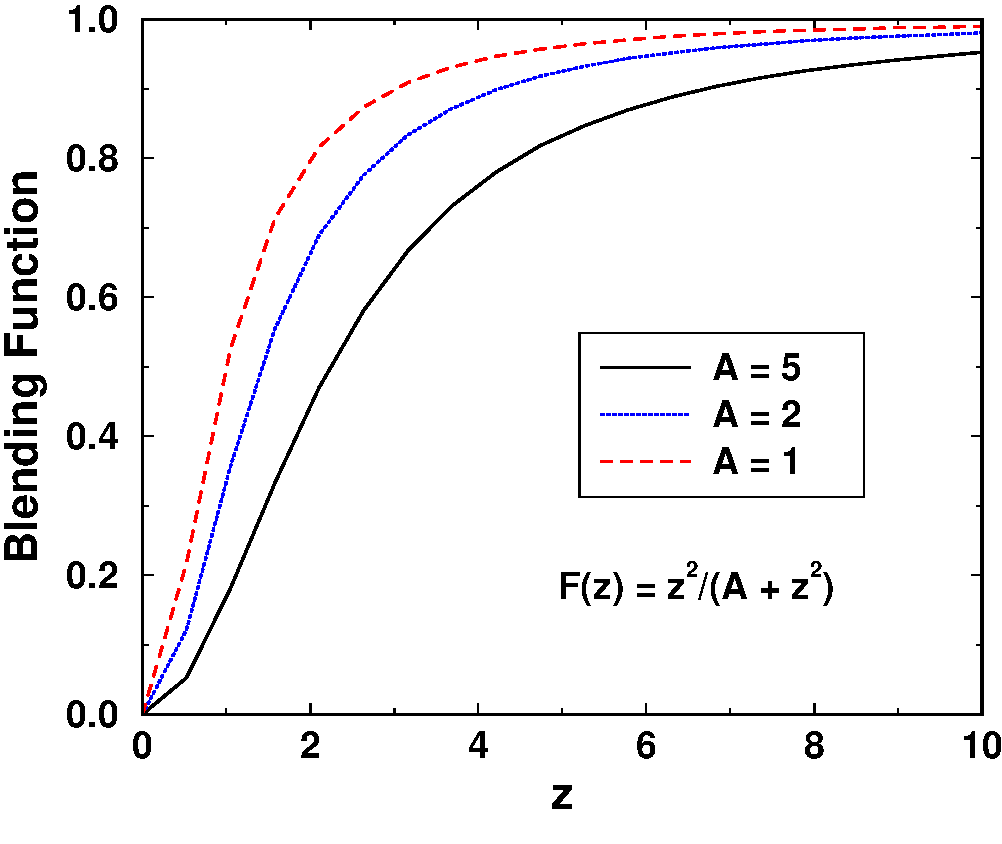
\includegraphics[height=3.0in]{images/peclet}}
\vspace{0.1in}
\caption{Cell-Peclet number blending function (classic).}
\label{pec-blend}
\end{figure}
 
The upwind operator, $\phi_{upw}$ is computed based on a blending of the extrapolated
state (using the projected nodal gradient) and the linear interpolated state. Second 
or third order upwind is provided based on the value of $\alpha_{upw}$ blending
\begin{eqnarray}
 \phi_{upw} = \alpha_{upw}\tilde \phi^L_{upw} + \left(1-\alpha_{upw}\right)\phi_{cds}; \dot m > 0, \nonumber \\
             \alpha_{upw}\tilde\phi^R_{upw} + \left(1-\alpha_{upw}\right)\phi_{cds}; \dot m < 0.
\label{phiUpwindFull}
\end{eqnarray}
The extrapolated value based on the upwinded left ($\phi^L$) or right ($\phi^R$) state,

\begin{eqnarray}
  \tilde \phi^L_{upw} = \phi^L + d^L_j \frac{\partial \phi^L }{\partial x_j}, \nonumber \\
  \tilde \phi^R_{upw} = \phi^R - d^R_j \frac{\partial \phi^R }{\partial x_j}.
\label{advUpwLR}
\end{eqnarray}
%
The distance vectors are defined based on the distances between the L/R points and the integration point 
(for both edge or element-based),
\begin{eqnarray}
  d^L_j = x^{ip}_j - x^L_j, \nonumber \\
  d^R_j = x^R_j - x^{ip}_j. 
\end{eqnarray}
\label{distanceVec}
In the case of all transported quantities, a Van Leer limiter of the extrapolated value is supported
and can be activated withing the input file (using the solution options ``limiter'' specification).

Second order central is simply written as a linear combination of the nodal values,
\begin{equation}
 \phi_{cds} = \sum N^{ip}_k \phi_k.
\label{phiCentral}
\end{equation}
%
where $N^{ip}_k$ is either evaluated at the subcontrol surface or edge midpoint. In the case
of the edge-based scheme, the edge midpoint evaluation provides for a skew symmetric form
of the operator. 

The generalized central difference operator is provided by blending with the extrapolated values and 
second order Galerkin,
\begin{equation}
 \phi_{gcds} = \frac{1}{2} \left(  \hat\phi^L_{upw} + \hat\phi^R_{upw} \right),
\label{phi4th}
\end{equation}
where,
\begin{eqnarray}
  \hat\phi^L_{upw} = \alpha \tilde \phi^L_{upw} + \left(1-\alpha\right) \phi_{cds}, \nonumber \\
  \hat\phi^R_{upw} = \alpha \tilde \phi^R_{upw} + \left(1-\alpha\right) \phi_{cds}.
\label{advNew4th}
\end{eqnarray}
The value of $\alpha$ provides the type of psuedo fourth order stencil and is specified in the user
input file.

The above set of advection operators can be used to define an idealized one dimensional stencil denoted
by ($i-2$, $i-1$, $i$, $i+1$, $i+2$), where $i$ represents the particular row for the given transported
variable. Below, in Table~\ref{tab-stencil} the stencil can be noted for each value of $\alpha$ and $\alpha_{upw}$.


\begin{table}[h]
 \caption{Edge-based stencils for various combinations of $\alpha$ and $\alpha_{upw}$}
 \label{tab-stencil}
 \vspace{0.1in}
 \centerline{
  \begin{tabular}{|l|l|l|l|l|l|l|} \hline
    $i-2$             &  $i-1$           &  $i$            & $i+1$           &  $i+2$           & $\alpha$      & $\alpha_{upw}$ \\ \hline
    $0$               &  $-\frac{1}{2}$  &  $0$            & $+\frac{1}{2}$  &  $0$             & $0$           & $n/a$          \\ \hline
    $+\frac{1}{8}$    &  $-\frac{6}{8}$  &  $0$            & $+\frac{6}{8}$  &  $-\frac{1}{8}$  & $\frac{1}{2}$ & $n/a$          \\ \hline
    $+\frac{1}{12}$   &  $-\frac{8}{12}$ &  $0$            & $+\frac{8}{12}$ &  $-\frac{1}{12}$ & $\frac{2}{3}$ & $n/a$          \\ \hline
    $+\frac{1}{4}$    &  $-\frac{5}{4}$  &  $+\frac{3}{4}$ & $+\frac{1}{4}$  &  $0$             & $\dot m > 0$  & $1$ \\ \hline
    $0$               &  $-\frac{1}{4}$  &  $-\frac{3}{4}$ & $+\frac{5}{4}$  &  $-\frac{1}{4}$  & $\dot m < 0$  & $1$ \\ \hline
    $+\frac{1}{6}$    &  $-\frac{6}{6}$  &  $+\frac{3}{6}$ & $+\frac{2}{6}$  &  $0$             & $\dot m > 0$  & $\frac{1}{2}$ \\ \hline
    $0$               &  $-\frac{2}{6}$  &  $-\frac{3}{6}$ & $+\frac{6}{6}$  &  $-\frac{1}{6}$  & $\dot m < 0$  & $\frac{1}{2}$ \\ \hline
  \end{tabular}
 }
\end{table}

It is noted that by varying these numerical parameters, both high quality, low dissipation operators
suitable for LES usage or limited, monotonic operators suitable for RANS modeling can be accomodated.
